%% 
%% Copyright 2007, 2008, 2009 Elsevier Ltd
%% 
%% This file is part of the 'Elsarticle Bundle'.
%% ---------------------------------------------
%% 
%% It may be distributed under the conditions of the LaTeX Project Public
%% License, either version 1.2 of this license or (at your option) any
%% later version.  The latest version of this license is in
%%    http://www.latex-project.org/lppl.txt
%% and version 1.2 or later is part of all distributions of LaTeX
%% version 1999/12/01 or later.
%% 
%% The list of all files belonging to the 'Elsarticle Bundle' is
%% given in the file `manifest.txt'.
%% 
%% Template article for Elsevier's document class `elsarticle'
%% with harvard style bibliographic references
%% SP 2008/03/01

%\documentclass[preprint,12pt,5p,authoryear]{elsarticle}
\documentclass[10pt,authoryear,twocolumn]{article}
\usepackage[utf8]{inputenc}



\usepackage[colorlinks=true]{hyperref}	% Links
\usepackage{amsmath}
\usepackage{siunitx}	% Valores con unidades
	\sisetup{range-phrase = --}
	\sisetup{separate-uncertainty = true}
	\sisetup{allow-number-unit-breaks = true}
	\sisetup{tight-spacing = true}
\usepackage{soulutf8}		% Resaltado, subrayado y demás
	\DeclareRobustCommand{\hlcolor}[2][yellow]{{\sethlcolor{#1}\hl{#2}}}

\usepackage{amssymb}
\DeclareSIUnit\ppm{ppm}
\DeclareSIUnit\pixel{px}
\DeclareSIUnit\arb{AU}

\newcommand{\I}{\mathrm{i}}
\newcommand{\FE}{\textit{FE}}
\newcommand{\Sum}{\textit{Sum}}
\newcommand{\R}{\textit{R}}
\newcommand{\DefX}{\textit{DefX}}
\newcommand{\DefY}{\textit{DefY}}
\newcommand{\low}[1]{\textsubscript{#1}} % Subíndices en modo texto


% No importar las sigiuentes librerías en caso de usar la plantilla de Elsevier
\usepackage{authblk}
\usepackage{graphicx}
\usepackage[
    backend=bibtex,
    citestyle=numeric-comp,
    bibstyle=numeric,
    natbib=true,
    date=year,
    sortlocale=en_US,
    url=true, 
    doi=true,
    hyperref=true,
    backref=true,
    backrefstyle=three
]{biblatex}
\addbibresource{BibLaTex.bib}


\begin{document}


%% Formato Elsevier


%\journal{Journal of Petroleum Science and Engineering}
%
%\begin{frontmatter}
%
%\title{Online oil-in-water and suspended solids measurement device based on thermal lens spectrometry and forward scattering}
%
%\author[AddressDF]{Axel Lacapmesure\corref{Corr1}} \ead{axel.lacapmesure@gmail.com}
%\author[AddressYTEC]{Darío Kunik}
%\author[AddressFIUBA]{Oscar E. Martínez}
%
%\address[AddressDF]{Departamento de Física, Facultad de Ciencias Exactas y Naturales, Universidad de Buenos Aires, Ciudad Autónoma de Buenos Aires, Argentina}
%\address[AddressYTEC]{YPF Tecnología S.A., Buenos Aires, Argentina}
%\address[AddressFIUBA]{Laboratorio de Fotónica, Facultad de Ingeniería, Universidad de Buenos Aires, Ciudad Autónoma de Buenos Aires, Argentina}
%
%\cortext[Corr1]{Corresponding author}
%
%
%
%\begin{abstract}
%
%\end{abstract}
%
%
%\begin{keyword}
%
%\end{keyword}
%
%\end{frontmatter}

%% Formato típico

\title{Online oil-in-water and suspended solids monitor based on thermal lens spectrometry and forward scattering}

\author[a]{Axel Lacapmesure \thanks{Corresponding author: axel.lacapmesure@gmail.com}}
\author[b]{Darío Kunik \thanks{dario.kunik@ypftecnologia.com.ar}}
\author[c]{Oscar E. Martínez \thanks{omartinez@fi.uba.ar}}
\affil[a]{\footnotesize Departamento de Física, Facultad de Ciencias Exactas y Naturales, Universidad de Buenos Aires, Pabellón I, Ciudad Universitaria, Intendente Güiraldes 2160, C1428EGA Ciudad Autónoma de Buenos Aires, Argentina}
\affil[b]{YPF Tecnología S.A., Av. del Petróleo Argentino 900-1198, Berisso, 1923 Buenos Aires, Argentina}
\affil[c]{Laboratorio de Fotónica, Facultad de Ingeniería, Universidad de Buenos Aires, Av. Paseo Colón 850, C1063ACV Ciudad Autónoma de Buenos Aires, Argentina}

\maketitle

\begin{abstract}

A novel system for continuous online monitoring of both oil-in-water and suspended solids based on thermal lens spectroscopy and forward scattering is presented. The technique measures the concentration of dissolved hydrocarbons and simultaneously detects single oil droplets and suspended particles separately. The device was tested with injection water from an on-field water treatment plant, through which hydrocarbon concentration were measured with a minimum resolution of \SI{0.02}{\ppm} and precision better than \SI{5}{\percent} in the range up to \SI{100}{\ppm}. Particle detection was tested on artificial samples of polystyrene spheres acting as absorption and scattering centers simulating oil droplets and suspended solids respectively. We show that their concentration can be determined in the range up to \SI{3000}{particles\per\milli\litre} while also distinguishing particles of different sizes.

\end{abstract}

\section*{Keywords}
Injection water quality; Online monitor; Oil-in-water; Suspended solids; Thermal lens spectroscopy; Light scattering

%% main text

%Falta:
%\begin{itemize}
%\item Mostrar señal típica (quizás con histograma, moda y dispersión) y detección de picos.
%\end{itemize}



\section{Introduction}
\label{Introduction}

Maintaining high injectivities over long periods of time is extremely important in all water injection projects. With the increasing stream of oilified-produced water and the tightening of environmental regulations, produced water reinjection has become one of the best options to manage large volumes of waste water in an economically attractive and environmentally safe way \citep{Furtado2005,Souza2005,Abou-Sayed2007}. However, even after water treatment, the complexity of produced water composition leads to important difficulties for injection processes regarding plugging, corrosion and permeability impairment among other problems. It has been found that induced injectivity decrease is more severe when both oil droplets and suspended solids are present in injection water because they interact jointly with the porous medium leading to particle deposition, pore bridging and internal or external cake formation \citep{Bennion1998,Chaveteau1998,Reousseau2008,Ali2009}. In all cases, the ratio between particle size and pore throat and the particle and oil concentrations are critical parameters since they have an important influence on the magnitude and time scale of permeability reduction \citep{vanderBroek1999,Ali2007,Buret2010}, thus making water quality monitoring essential for prediction and control of injectivity impairment and for the evaluation of water treatment processes.

%Water quality monitoring is essential for most stages of oil production. In all water injection projects such as secondary oil recovery, maintaining high injectivities over long periods of time is extremely important, but depositions of organic material and suspended solids from injection water produces well plugging that reduces oil production \hlcolor{[REFERENCIAS]}. In tertiary oil recovery, the manufacturing of polymers for chemical injection typically requires high quality water since the presence of hydrocarbons may trigger the agglomeration of solids which also induce well plugging \hlcolor{[REFERENCIAS]}. Well cleaning demands expensive procedures and suspends oil production, so water quality monitoring is necessary for both prevention and to evaluate water treatment processes. Additionally, controlling water quality is a requirement in offshore oil recovery, where wastewater is usually poured onto the sea and hence strict regional regulations controls its allowed hydrocarbon concentrations \hlcolor{[REFERENCIAS]}.

Water quality analysis can be conducted on field and outside field, and typically comprises taking a sample of the water under study and then detect and measure the concentration of its components by means of diverse procedures that usually involve chemical extraction and/or separation techniques. While these analyses are fundamental since they can provide results in absolute units and allows for comparison of results obtained from different installations, they typically demand long times (as long as several weeks) until results are available and thus are impracticable for process trending and detection of process deviation, which requires online monitoring instead. In the last decades, alternative techniques based on optical phenomena were developed and implemented aiming to respond to this need, with some of them currently available in the market. Below we summarize the most noteworthy examples with some of the difficulties they present.

Scattering based methods detects the angular distribution of light scattered by oil droplets and other suspended particles contained in the sample. These systems don't account for dissolved hydrocarbons and showed difficulties to differentiate suspended particles of same size but different composition \citep{He2003}. Fluorescence based methods detect the fluorescence emission from aromatic components in the sample when it is irradiated with UV light. In this case the sensitivity is highly dependent on the relation between aromatics hydrocarbons and the rest of the oil components \citep[ch. 4]{Parker1987}, and both competing electronic decay processes and quenching alters the overall response at different concentration levels, thus introducing nonlinearities \citep{Downare1995}. Similarly a surface enhanced Raman scattering sensor was proposed for detection of polyciclic aromatic carbons such as anthracene and pryrene \citep{Kolomijeca2011}, but this method is also dependent of the relative concentration of aromatics hydrocarbons. Additionally some methods based on photoacustic sensors and UV/NIR light absorption were reported, but none has shown reliable at concentrations lower than \SI{50}{\ppm} \citep{Freeborn1998,He2003}. In all cases, none of the proposed methods allows for a separated characterization of both suspended solids and oil concentrations.

Alternativelly, techniques for sample characterization based on thermal lens effects had been extensively developed since the first report of thermal lens effect by Gordon in 1965 \citep{Gordon1965}, leading to some of the most sensitive methods for thermophysical and chemical analysis, such as thermal lens spectroscopy \citep{Franko2010,Liu2016}. This technique is based on the measurement of the local refractive index variation induced by the light absorption and subsequent heating of an irradiated sample, which constitutes an optical lens. Its application on chemical analysis is possible since the power of the lens depends on the concentration of absorbing components, hence allowing detection of absorbances as low as \SI{d-7}{\arb} \citep{Proskurnin2015}. In comparison to other optical methods, thermal lens based techniques are intrinsically less sensitive to scattering effects, making it ideal for characterization of heterogeneous samples or colloidal solutions while also offering diverse and versatile configurations in order to exploit the photochemical properties of the sample. Thermal lens spectrometry has proven useful in diverse high sensitivity chemical trace detection and analysis \citep{Sikovec1996,Franko2010}, and it can also be coupled to chemical separation systems or microfluidic injection systems for enhanced selectivity \citep{Liu2016}. \\

In this work we present and discuss a novel water quality monitoring system for both oil-in-water and suspended solids measurement based on thermal lens spectrometry and forward scattering. The device comprises a thermal lens spectrometer with a pump and probe beam configuration where both the power of the thermal lens and the optical transmission of the probe beam are measured. Transmission signal provides information about both absorbing (i.e. hydrocarbons) and scattering (i.e. suspended solids and oil droplets) components of the sample, while thermal lens signal only provides information about absorbing components, thus allowing to measure the concentration of dissolved oils as well as to detect oil droplets and suspended solids separately. Along our work the device was tested with water samples from on-field water treatment facilities and also with artificial colloidal solutions made for controlled tests. The whole system allowed a continuous and fast characterization of the sample with measurement duration of about \SI{200}{\second}, and since sample preparation isn't required and its configuration is compatible with a flow-through system, the device proves ideal for usage as an online monitor that can be incorporated into injection flowlines.








\section{Experimental}
\label{Experimental}

The device uses a thermal lens spectrometer configuration with two collineal beams, namely a high-power, intensity modulated pump beam and a low-power, CW probe beam. The configuration consists of two main distinct sections: the thermal lens generation sector, which essentially comprises the lasers and the sample, and the focus error detection system, through which simultaneous measurement of both the thermal lens power and the optical transmission of the probe beam were made \citep{Domene2017}.

To generate the thermal lens, both beams are focused on a sample contained in a flourometer cuvette. Along the beam propagation through the sample, the pump beam energy is partially absorbed and dissipated as heat, thus locally increasing the temperature of the medium and generating a refractive index profile. If the temperature elevation is smooth enough, the refractive index profile forms an optical lens that defocuses the probe beam due to the negative sign of the thermo-optic coefficient of water. In the low-absorption regime, the power of this thermal lens is proportional to the total energy absorbed, hence allowing to perform high-sensitivity absorbance measurements by characterizing the probe beam defocusing. Also, in order to achieve an efficient oil-in-water detection it is necessary to choose a pump wavelength that gives a high contrast between absorption from oil and water. Therefore we chose a \SI{532}{\nano\metre} wavelength, at which the absorption coefficient of oil is typically \SI{6}{} to \SI{7}{} orders of magnitude larger than for water, and also high-power lasers are available.

Subsequently the probe beams enters the focus error detection system, where both the change of focus and its transmitted power are measured. The system comprises a pair of cylindrical lenses whose axes are oriented orthogonally, therefore creating an astigmatic focused beam with waists in the horizontal and vertical directions at different planes. There is an intermediate plane at which the beam is circular, and the presence of a thermal lens that defocuses the probe beam moves this plane along the optical axis. A four-quadrant photodiode was used to measure the beam ellipticity through generation of a focus error \FE{} signal \citep{Domene2017}. Additionally, the total transmitted power is measured by summing the signals of all quadrants, enabling the usual measurement of the extinction coefficient through transmission. Normalizing \FE{} with the transmitted power leads this signal to respond only to beam geometry independently of its intensity, and thus characterizing the probe beam defocusing: \FE{} is zero when placed in the plane where the beam is circular, but in presence of a thermal lens, the beam on that plane becomes elliptical and leads to a nonzero \FE{} signal. \\

%A four-segment photodiode was used to measure the beam transverse power distribution along the horizontal and vertical directions. This allows to generate a focus error signal
%\begin{equation}
%	\FE{} = (A+C)-(B+D),
%\end{equation}
%where $A$ and $C$ corresponds to the horizontal segments and $B$ and $D$ corresponds to the vertical segments. Normalization with the incident power leads \FE{} to respond only to geometrical factors independently of the probe laser power, measuring the beam ellipticity and thus characterizing the beam defocusing: when placed in the plane where the beam is circular, the incident power on all segments is the same and \FE{} is zero, but in presence of a thermal lens, the beam on that plane becomes elliptical and unbalances the incident power on the horizontal and vertical segments of the detector, giving a nonzero focus error signal. Additionally, the total transmitted power is measured by summing the signals of all quadrants, enabling the usual measurement of the extinction coefficient through transmission. \\

\begin{figure*}[h]
	\centering 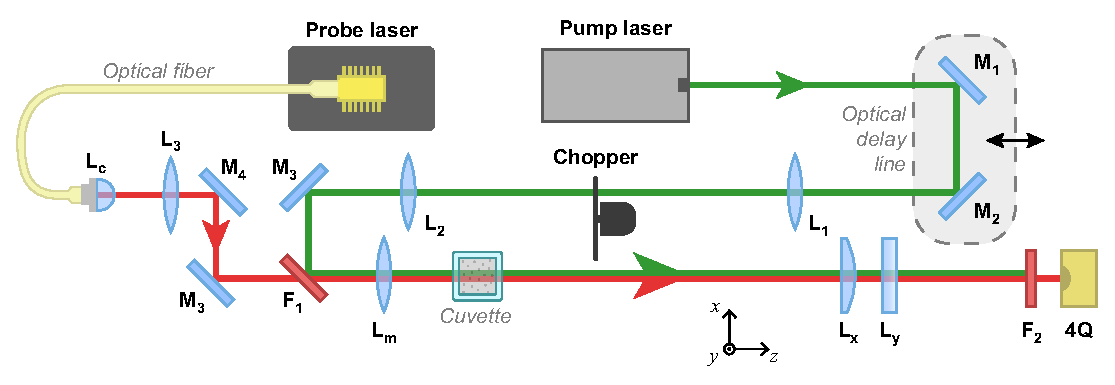
\includegraphics[width=\textwidth]{Figuras/1_Setup.eps}
	\caption{Experimental setup. \textbf{M\low{1} to M\low{5}:} mirrors for beam alignment. \textbf{L\low{c}:} probe collimating lens. \textbf{L\low{1} to L\low{3}:} pump and probe optics, in addition with \textbf{L\low{m}}. \textbf{F\low{1} and F\low{2}:} \SI{700}{\nano\metre} longpass filter for beam coupling and pump filtering respectively. \textbf{L\low{x} and L\low{y}:} cylindrical lenses. \textbf{4Q:} four-quadrant photodiode.}
	\label{fig:Experimental}
\end{figure*}

Figure \ref{fig:Experimental} shows a simplified diagram of the experimental setup. The sample was contained in a PMMA fluorometer cuvette with a \SI{10}{\milli\metre} optical path. As a light source for the pump beam, we used a doubled Nd:YAG laser \emph{Coherent} model \emph{Compass 315M-100} with a \SI{100}{\milli\watt} maximum output power at a \SI{532}{\nano\metre} wavelength, and which was controlled by a driver provided by the manufacturer. The beam was then modulated by a chopper at a frequency of \SI{350}{\hertz}, which was much faster than the characteristic times of heat transfer by convection and diffusion processes, hence simplifying the thermal lens dependence by neglecting these effects. For the probe beam, a fiber-coupled laser diode \emph{QPhotonics} model \emph{QFLD-780-100S} was used, which provided a high quality gaussian beam with nearly \SI{500}{\micro\watt} power in the sample at a \SI{780}{\nano\metre} wavelength.

The pump beam focusing optics was chosen to obtain a confocal parameter on the sample similar to the optical path of the cuvette. In order to minimize aberrations introduced by the edges of the thermal lens, the probe beam focusing optics was chosen to maximize the path length over which the probe beam was smaller than the pump beam. Altogether, this led to beam waists of \SI{55}{\micro\metre} for the pump beam and of \SI{33}{\micro\metre} for the probe beam. To control the displacement between both waists along the optical axis, the pump beam passed through a simple optical delay line comprised of two mirrors on a translation stage.

The focus error detection system comprised two \SI{75}{\milli\metre} focal length cylindrical lenses and a \SI{1}{\milli\metre^2} total active area four-quadrant photodetector. The system has two free parameters, namely the separation between the lenses and the distance from the lenses to the sample, which were chosen in order to optimize the sensitivity of the \FE{} signal in the presence of a thermal lens. To do so, the beam propagation and the \FE{} signal were simulated as a function of those parameters, and the optimal configuration within mechanical limitations was chosen. Afterwards, the detector was positioned on the plane where the probe beam was circular. In practice, the \FE{} signal was obtained from the signal of all quadrants by a series of summing op-amps circuits and then acquired and processed by a PCI lock-in amplifier \emph{Anfatec} model \emph{AMU 2.4} in order to filter the harmonic component at the pump modulation frequency. Additionally, the signal from each quadrant was acquired by a 16 bits, \SI{1}{\mega\hertz} bandwidth, PCI DAQ board \emph{IOtech} model \emph{DaqBoard/3001}. This allowed to measure the total transmitted power by summing the signals from all quadrants through software and hence to normalize \FE{} signal, and also to generate additional auxiliary signals. \\

With our prior understanding of the system we can already anticipate the signals responses in the presence of a sample of injection water. On the one hand, the absorbing components dissolved in water along with water itself will contribute to generate a thermal lens distributed over the irradiated volume, therefore increasing the thermal lens channel base level and decreasing the transmission channel base level due to bulk light absorption. To extract the contribution to thermal lens from dissolved components we compute the mode of the normalized thermal lens signal, which gives the absorption base level of the sample. On the other hand, suspended particles such as solids or oil droplets with sizes comparable to the beams waist will pass through the beams and alter the response above described. If the particle does not absorbs the pump radiation, it will act as a scattering center and momentarily decrease the transmitted power, which will be observed as a negative peak on transmission channel. If the particle does absorb the pump radiation it will also generate a thermal lens located around itself and thus defocus the probe beam even more, which will be observed as an additional positive peak in the thermal lens channel. To detect the contribution on each signal from suspended particles we use a peak detection algorithm developed on \emph{Matlab} that compares the signal fluctuations with those obtained with a sample of pure demineralized water, obtaining a time series of positive or negative peaks for each channel. In our work, these measurements were performed in a post-processing stage, but they also can be conducted on real-time processing.

Our experiments were designed and conducted to study the system behavior considering the above discussed preliminary analysis. To do so, we had two master samples taken from an injection well facility located in Comodoro Rivadavia, Argentina. The first one, which we will refer as IW100, is a sample of the injection water that consists on treated produced water, and had oil-in-water concentration of at least \SI{100}{\ppm}. The second one, which we will refer as IW10, is a sample of the water used for manufacturing of polymers used in chemically-enhanced extraction. It consists of the same injection water with further treatment and had a oil concentration of less than \SI{10}{\ppm}. The concentration values were given by the company that took the samples and performs water quality analysis periodically on this well. Additionally, to study the system behavior with controlled samples when analyzing the suspended particles, we prepared artificial colloidal samples from solutions of microspheres on demineralized water. To simulate suspended solids we used polystyrene spheres with a diameter of \SI{6}{\micro\metre}, while to simulate oil droplets we used polystyrene spheres dyed with a red pigment (thus absorbing at a \SI{532}{\nano\metre} wavelength) with diameters of \SI{6}{\micro\metre} and \SI{2}{\micro\metre}. We will refer to each master sample made as PS6 for the \SI{6}{\micro\metre} diameter undyed polystyrene spheres, and as PSD6 and PSD2 for the \SI{6}{\micro\metre} diameter and \SI{2}{\micro\metre} diameter polystyrene dyed spheres respectively. All spheres were manufactured by \emph{Phosphorex Inc.}








\section{Results and discussion}
\label{Results}

To study the system capability for characterizing dissolved components we performed serial dilutions of the IW100 and IW10 samples. First we progressively diluted IW100 on IW10, thus varying the oil concentration while preserving some of the water components. Secondly we diluted IW10 on demineralized water to extend the concentration range to lower values. For each iteration we performed a measurement with the same fixed parameters, namely lasers output power, acquisition length, lock-in and DAQ parameters, and then processed the data as above mentioned, obtaining the results plotted in figure \ref{fig:BulkAbsorption}.

\begin{figure}[t!]
	\centering 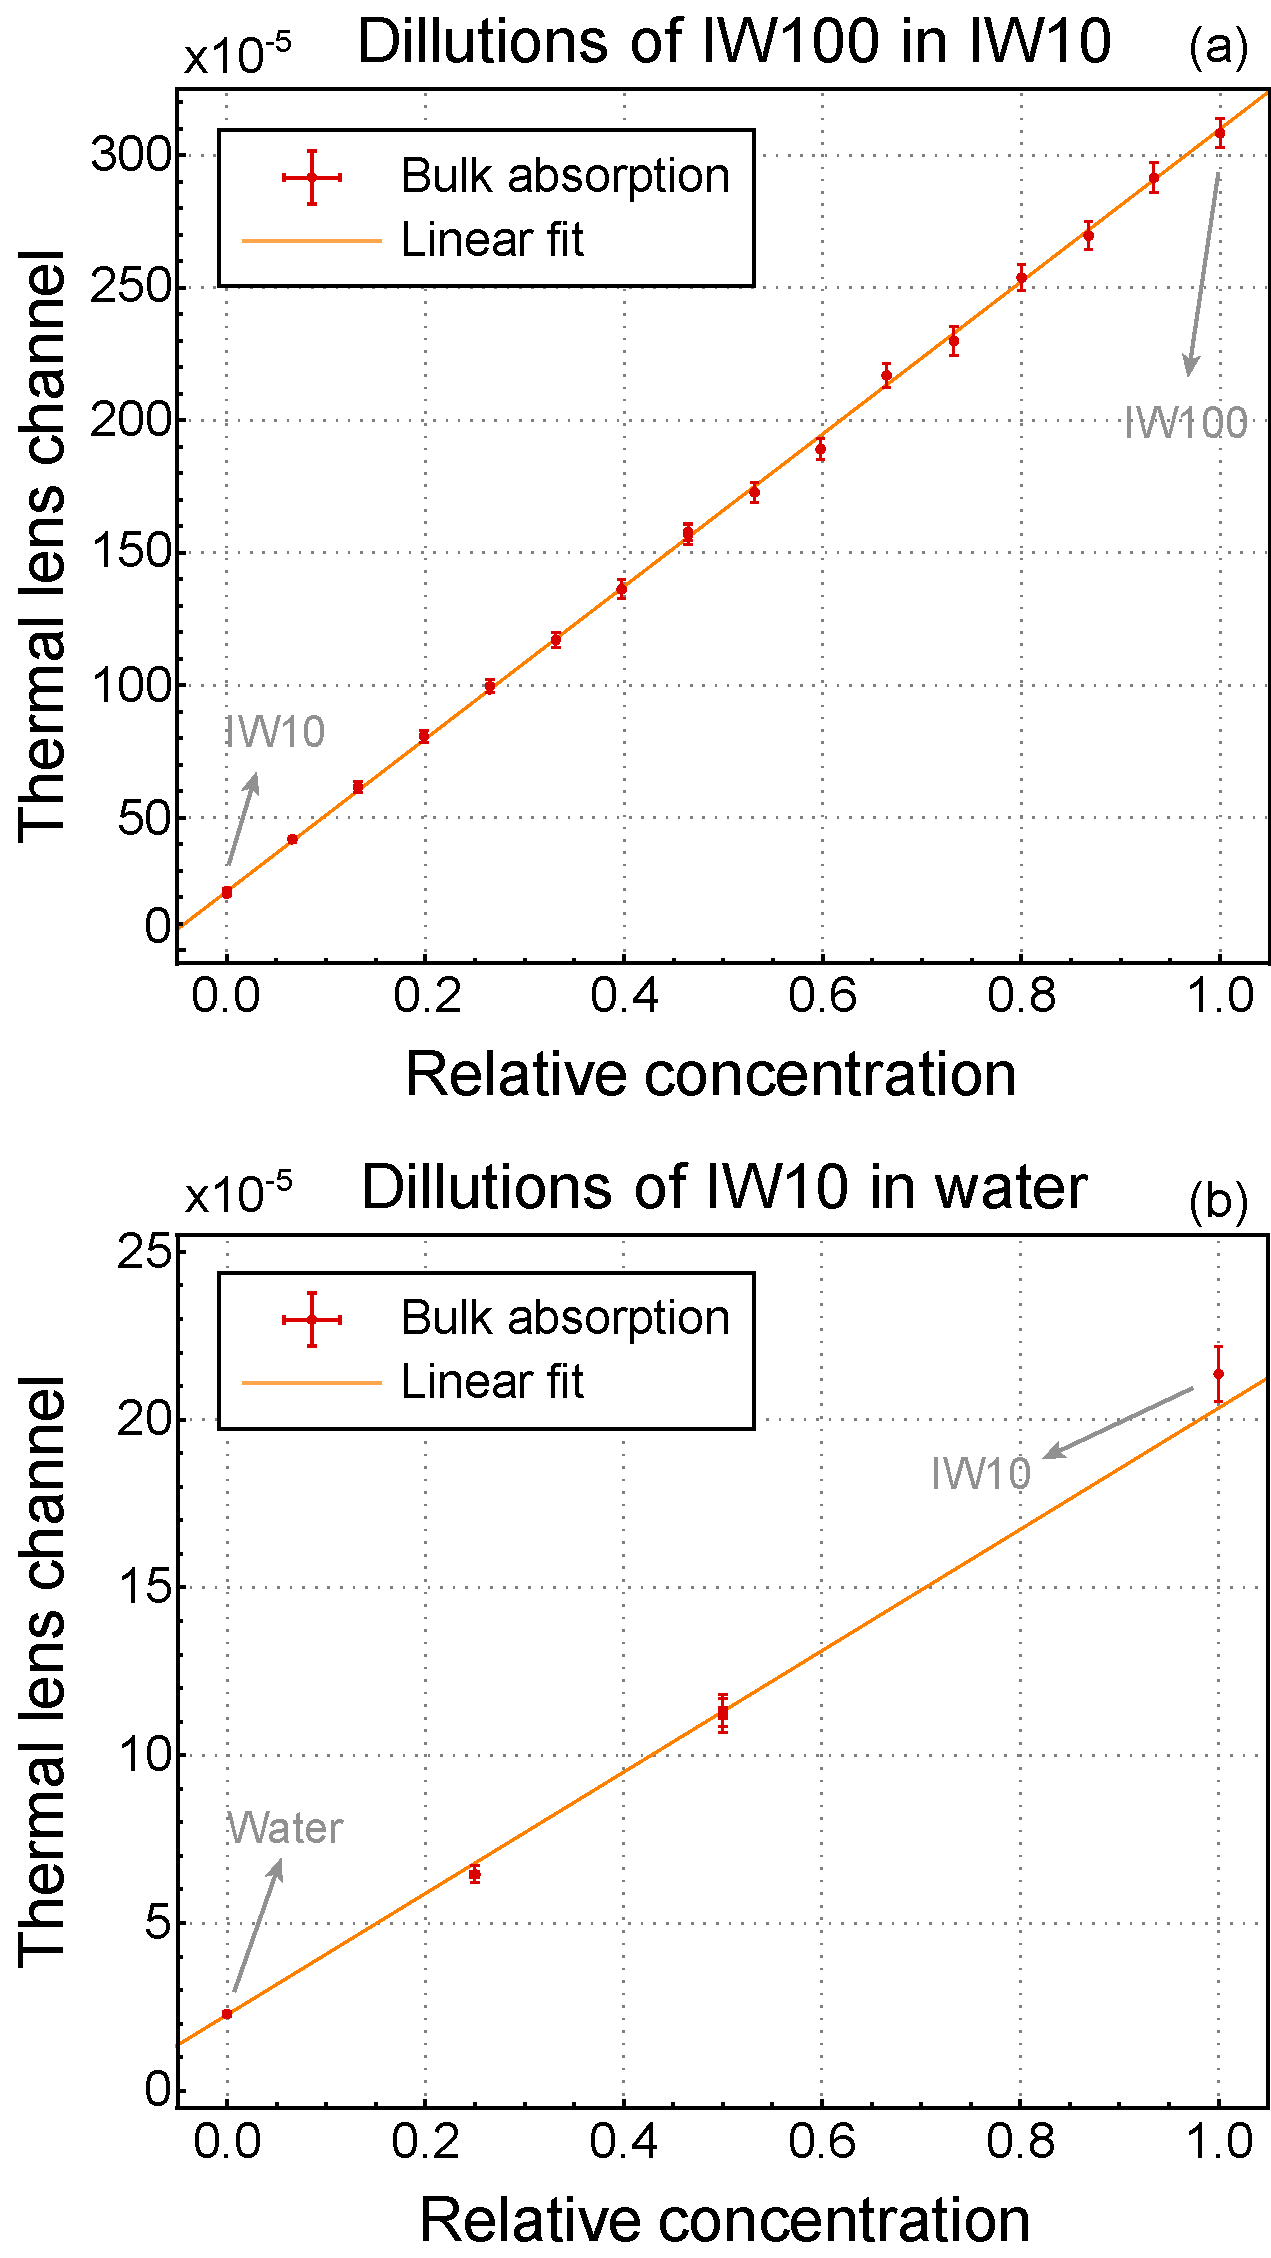
\includegraphics[width=.49\textwidth]{Figuras/IWvsC.pdf}
	\caption{Thermal lens signal from bulk absorption of dissolved components for serial dilutions of (a) IW100 on IW10 and (b) IW10 on demineralized water.}
	\label{fig:BulkAbsorption}
\end{figure}

The measurements for dilutions of IW10 on water allowed to study the performance of the device for injection water samples in the lowest absorption regime, recovering a linear response over the whole range of concentrations% and through a least squares linear regression on the data we obtained a slope of $\SI{1.8084(34)d-4}{}$, which is associated to the sensitivity of the device, and an y-intercept of $\SI{2.26(51)d-5}{}$, which corresponds to the signal level for a sample of pure water. Here, both uncertainties are taken as the \SI{95}{\percent} confidence intervals. With the adjusted slope it was possible to experimentally estimate the sensitivity of the device in therms of concentration by assuming an oil concentration of \SI{10}{\ppm} for the pure IW10 sample, resulting in a sensitivity of $\SI{1.8084(34)d-5}{\per\ppm}$. If the actual concentration of the master sample would be lower, our sensitivity would rise, therefore this value corresponds to a lower bound for the device sensitivity on these samples.
. A least squares linear regression was performed on the data, and from the adjusted slope it was possible to experimentally estimate the sensitivity of the device in therms of concentration by assuming an oil concentration of \SI{10}{\ppm} for the pure IW10 sample, resulting in a sensitivity of $\SI{1.8084(34)d-5}{\per\ppm}$ (note that \FE{} signal has no units after normalization with the transmission signal). If the actual concentration of the master sample would have been lower, our sensitivity would rise and therefore this value corresponds to a lower bound for the device sensitivity on these samples.

The ability to detect a certain amount of oil in the sample corresponds to the ability to distinguish its signal level from the background level due to absorption of pure water. Resolution is thus limited by both the contrast of water and oil absorption, which depends on specific oil absorption properties, and the signal fluctuations, which comprises mainly the noise and the variations induced by inhomogeneities in the sample composition. The measurement uncertainty thus depends on both the lock-in time constant %because a bandwidth reduction increases signal-to-noise ratio, but it also depends on the
and the acquisition duration, improving for longer acquisitions since they allow a better reconstruction of the signal distribution and a more reliable calculation of the mode. We measured the variance of the mode as a function of these parameters %acquisition length for a IW100 sample at fixed lock-in time constants, and observed that it remained constant for lengths larger than \SI{200}{\s}. %the mode dispersion diminishes from the initial signal variance to approximately 8 times less, and then remained constant for longer acquisitions. We
and then take the resolution of the device as the variance for an acquisition length if \SI{200}{\s} and time constant of \SI{1}{\s}. We do so independently of the sample by taking into account only the fluctuations introduced by the system noise (i.e. without the fluctuations due to inhomogeneities in the sample composition), obtaining a resolution of \SI{0.02}{\ppm}.% for the acquisition parameters used in our measurements.

Additionally, the dilutions of IW100 in IW10 allowed us to cover the range of concentrations of interest for most injection and polymer manufacturing purposes. In this case it was necessary to correct the signal levels due to degradation of the samples caused by the large time of exposure to light radiation. It should be mentioned that this effect was significant because the serial dilution protocol used spanned through several hours, but otherwise negligible on measurements of durations less than \SI{20}{\min} (as in an online operation). After corrections, we again observed a linear response that gives the calibration coefficients for this well once the exact oil concentration of the master samples are known. In all cases the measurement precision, obtained by the same way as the resolution but now taking into account all fluctuations, was better than \SI{5}{\percent}, being mostly limited by the fluctuations introduced by the sample inhomogeneous composition. Hence after proper calibration, an oil concentration around \SI{10}{\ppm} could be determined with an uncertainty better than \SI{0.2}{\ppm}. \\

When studying the system capability for particles and emulsion characterization, firstly the peak series for each solution of spheres in water was calculated and compared with a demineralized water reference, which also showed some peaks due to the presence of suspended particles. We observed that the amount of peaks detected agreed with the expected behavior of the signals described in our preliminary analysis. The undyed spheres, which acted only as scattering centers, showed \SI{40}{} times more negative peaks detected than for water, while we did not register any increase in peaks on the thermal lens channel, indicating not only the absence of absorption centers but also that the thermal lens signal is not affected by scattering losses. Additionally, the dyed spheres showed a similar increase for both negative peaks in the transmission channel and positive peaks in the thermal lens channel, indicating the spheres acted as both scattering and absorption centers.

To study the magnitude of the effects introduced by particles, we compute the height $p$ of each peak relative to the base signal level due to the bulk absorption of the sample. Figure \ref{fig:PeakHistogram} shows an histogram of the peak relative heights for all samples registered at (a) the transmission channel and (b) the thermal lens channel. When comparing particles of different sizes, the negative peaks in transmission channel reveals that larger spheres produces a distribution of higher peaks. This is also shown by the calculated mean peak height, which was of \SI{19.9d-3}{} for the PSD6 sample and of \SI{17.5d-3}{} for the PS6 sample (absolute values of \SI{0.422}{\volt} and \SI{0.404}{\volt} respectively), while the PSD2 sample had a mean height of \SI{6.54d-3}{} (absolute height of \SI{0.140}{\volt}). As expected, there isn't any significant difference between the distributions for spheres of the same size in this channel, whether dyed or undyed, indicating that absorption losses are negligible in relation to the total incident power.

\begin{figure}[t!]
	\centering 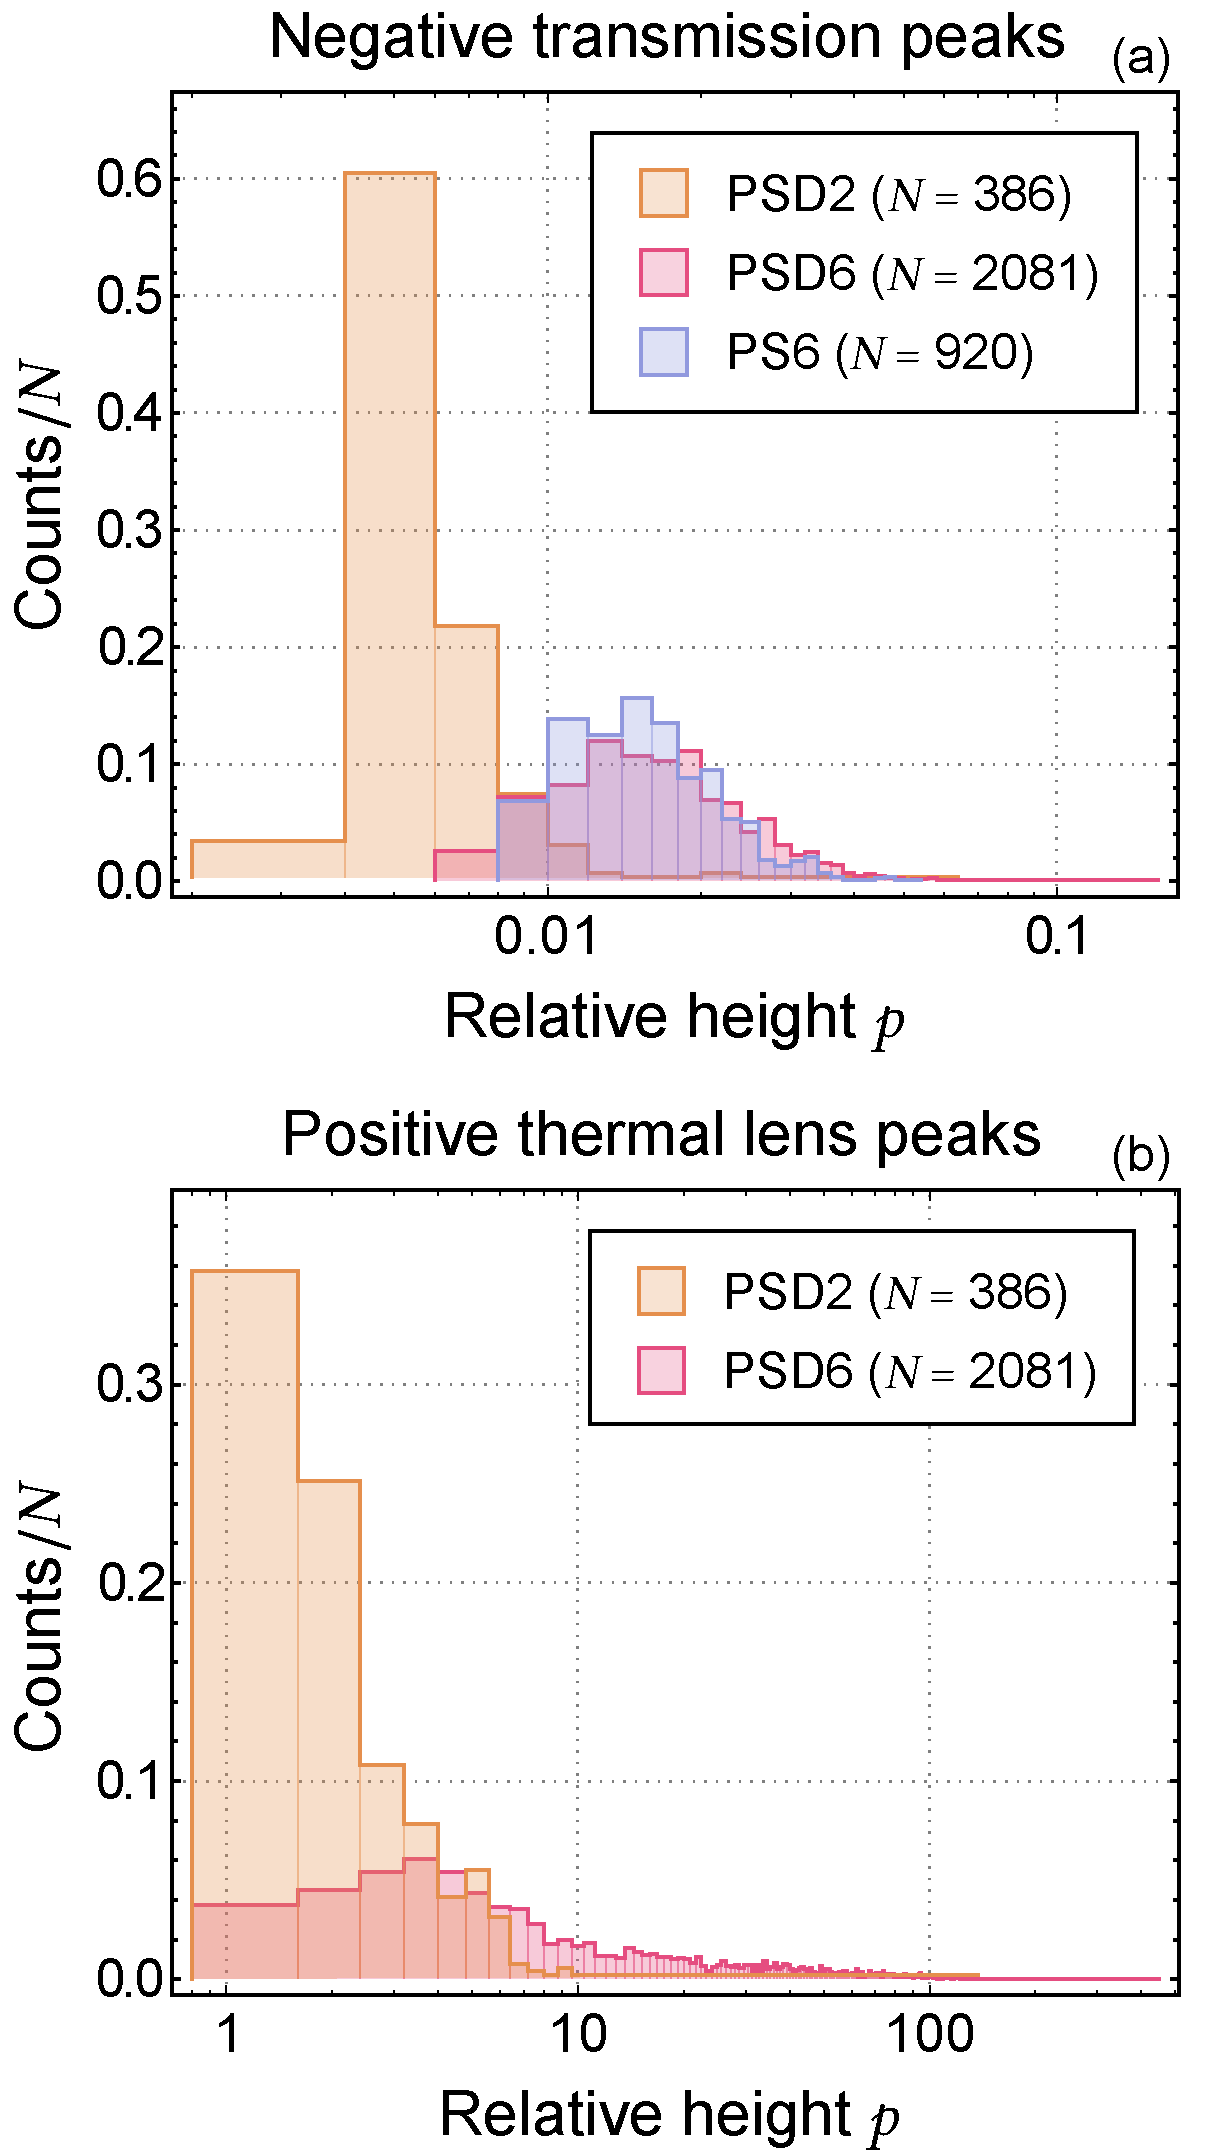
\includegraphics[width=.49\textwidth]{Figuras/PeakHeightDistribution.pdf}
	\caption{Histograms of relative peaks heights for (a) transmission channel and (b) thermal lens channel. On each case, counts are normalized to the total number of peaks detected $N$.}
	\label{fig:PeakHistogram}
\end{figure}

From figure \ref{fig:PeakHistogram} (b) we can make a similar analysis regarding the thermal lens channel, where we excluded the PS6 sample since it did not produce a significant amount of peaks on this signal. Here again we observe a distribution of peaks with larger heights for the solution with bigger spheres, which is also consistent with the calculated mean peak heights of \SI{2.86}{} for PSD2 sample and \SI{24.8}{} for PSD6 sample (absolute heights of \SI{1.00d-4}{} and \SI{7.74d-4}{} respectively). Considering that the thermal lens channel is insensitive to scattering from a single particle, the information provided by both channels is complementary and allows to differentiate suspended solids and oil droplets not only by their pigmentation but also by their size, since the peak heights correlates with their scattering or absorption cross section depending on the channel. It should be noted that peak detection is much more improved on the thermal lens channel, where peak prominence is several orders of magnitude larger than in transmission channel. This is due to both the better signal-to-noise ratio in phase-sensitive detection and the choice for a pump wavelength in the water absorption minimum, resulting in a higher contrast on the signal and therefore an efficient peak detection that enhances characterization of the absorbing components in the sample. \\

Particles concentration can be determined by studying the frequency of peaks. Assuming a solution of ideal and statistically independent particles and for concentrations low enough to consider the probability of finding one particle in the sample volume negligible, the passage of particles through the beams follows a Poisson statistics in which the interarrival time $\Delta$ between particles passing through the beams has a probability distribution
\begin{equation}
	P\left(\Delta > t\right) = \exp\left( -b t \right),
\label{eq:InterarrivalTimesPD}
\end{equation}
with $b$ being the reciprocal mean interarrival time, i.e. $\left\langle \Delta \right\rangle = 1/b$. We verified this behavior by computing the cumulative distribution probability of $\Delta$ for both the negative peaks of transmission channel and positive peaks of thermal lens channel, obtaining a probability distribution that agrees with \ref{eq:InterarrivalTimesPD} for values of $\Delta$ greater than the minimum interarrival time $\Delta_{min}$ our system could resolve. Here, $\Delta_{min}$ was limited mainly by the average peak width, the time constant of the lock-in amplifier and the fact that our system can't distinguish between one or many particles in the sample volume.

\begin{figure}[t!]
	\centering 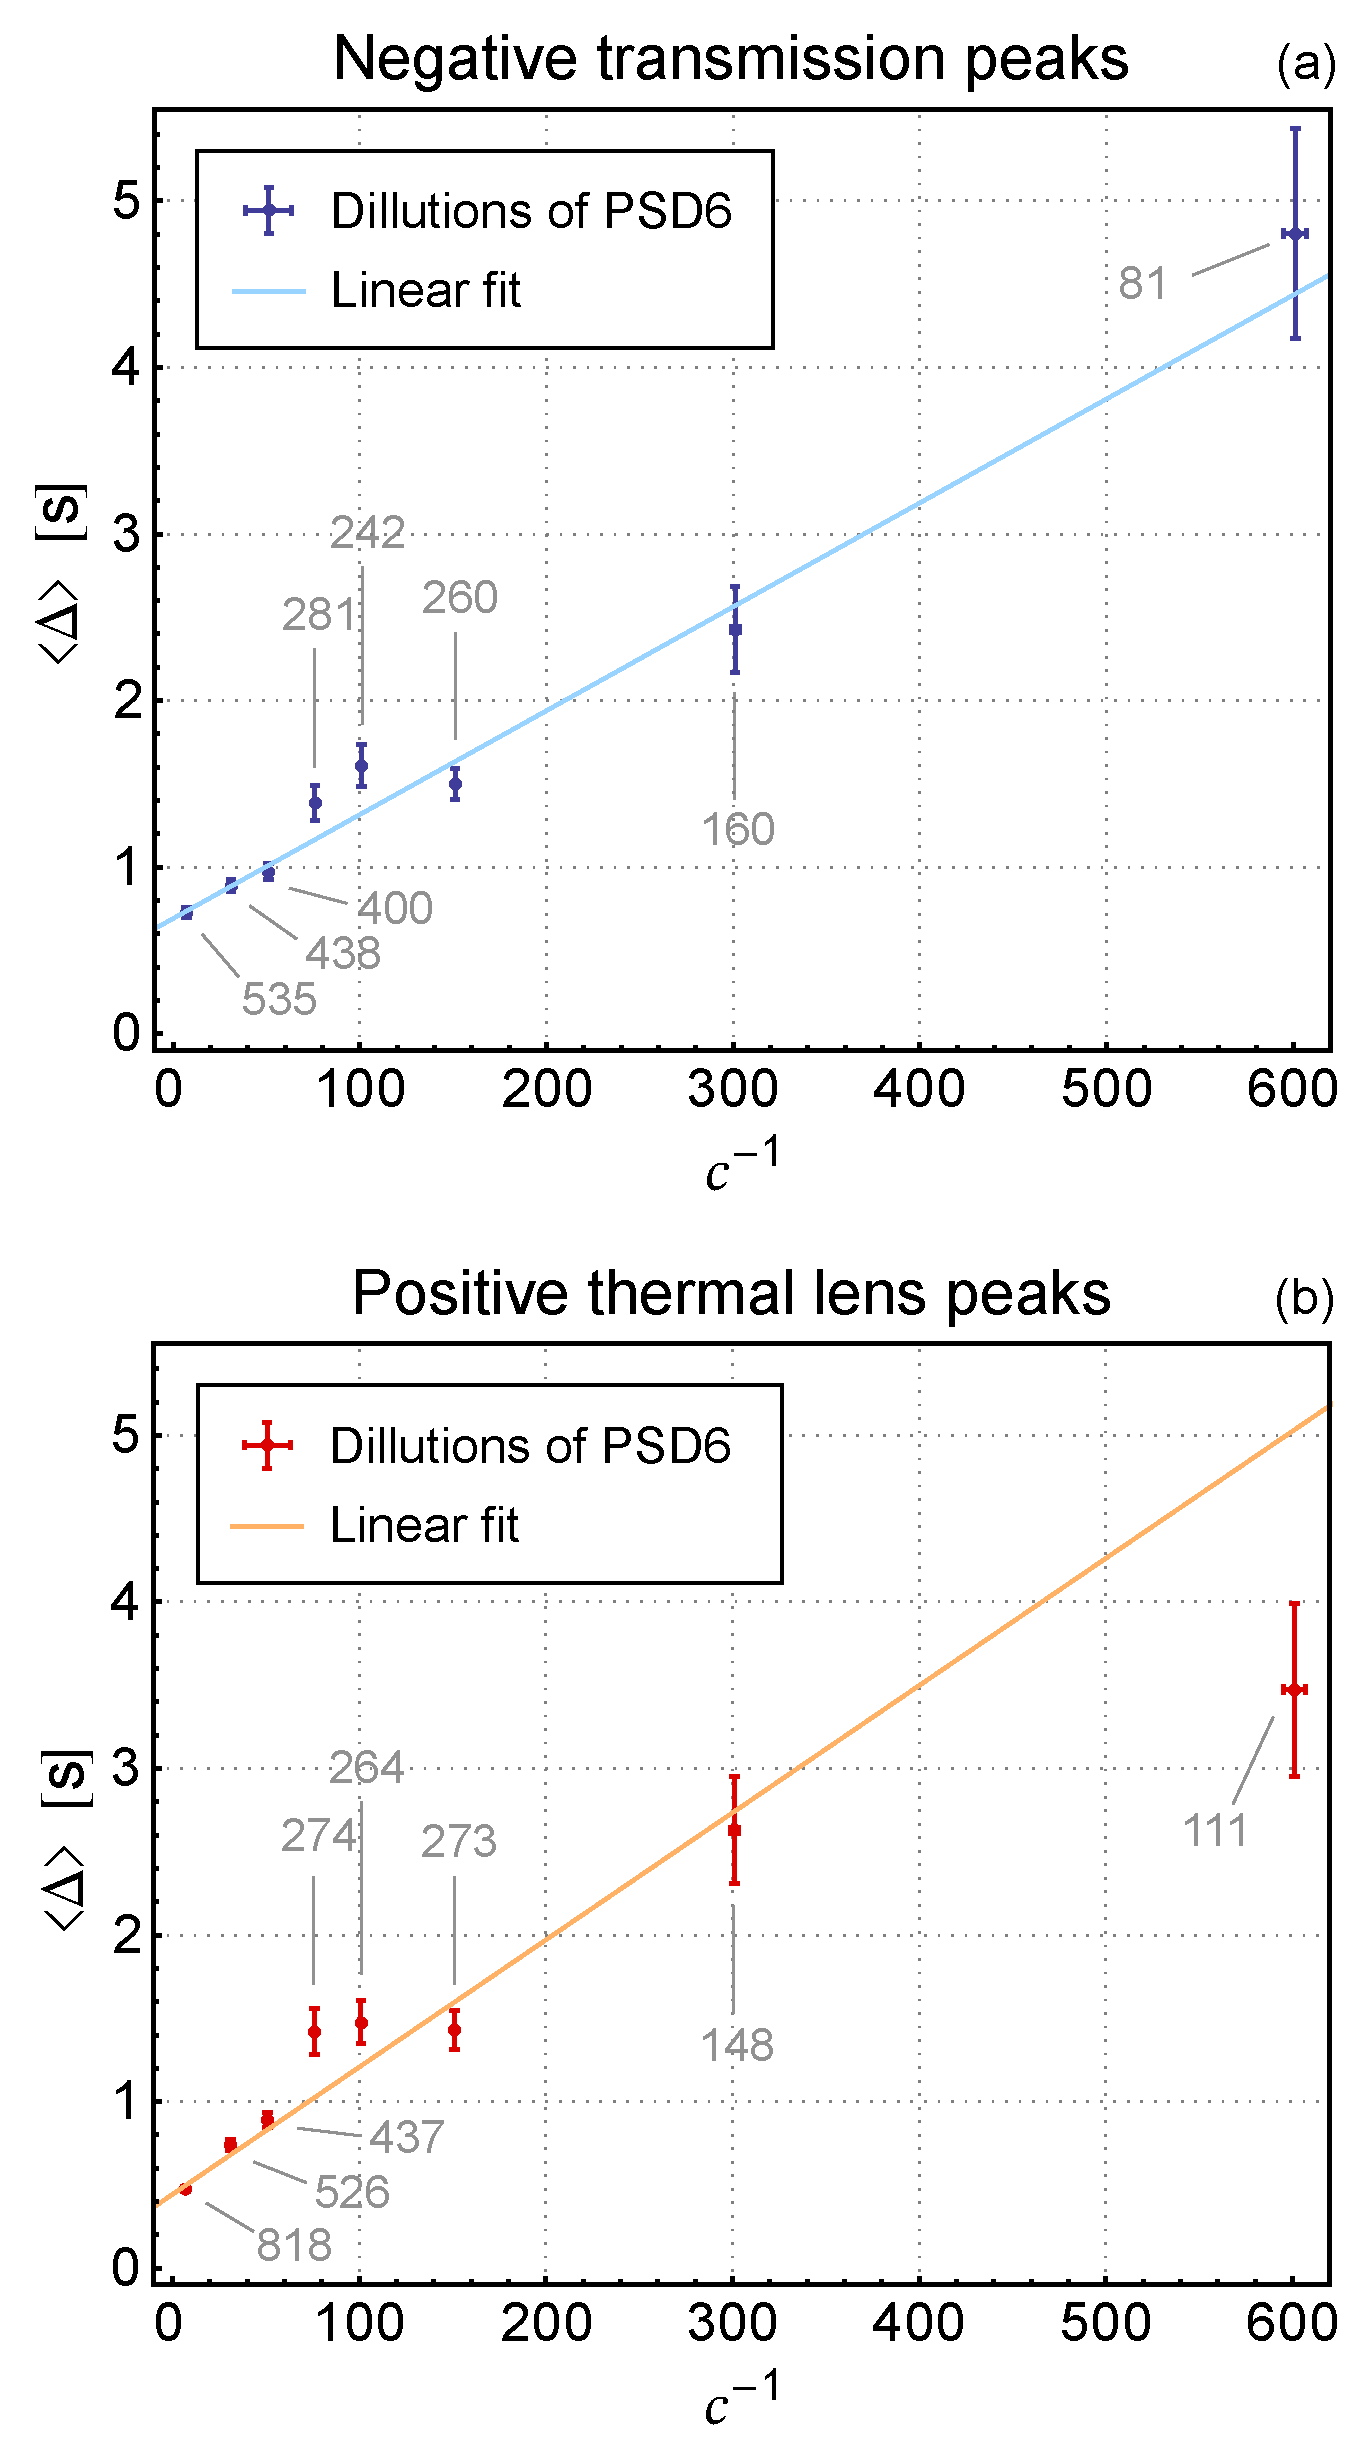
\includegraphics[width=.49\textwidth]{Figuras/InterarrivalTimes.pdf}
	\caption{Mean interarrival times of (a) peaks on transmission channel and (b) peaks on thermal lens channel obtained for serial dilutions of PSD6 on demineralized water, plotted against the reciprocal relative concentration $c$. Along with data points, the number of peaks detected for each dilution is indicated.}
	\label{fig:InterarrivalTimes}
\end{figure}

Under previous assumptions, it's fairly simple to derive from first principles an expression for the parameter $b$, obtaining
\begin{equation}
	b = 2 w_0 l u_\perp C,
\label{eq:bParamenter}
\end{equation}
where $l$ is the optical path of the cuvette, $2 w_0$ is the beam diameter, $u_\perp$ is the mean flow velocity in the direction transverse to the optical axis and $C$ is the absolute particle concentration (in terms of number of particles per unit volume). Hence equation \ref{eq:bParamenter} corresponds to the flow of particles through the sampling volume. It should be mentioned that this expression is valid for a collimated beam in a uniform transverse flow, but it could be extended for focused beams and an almost arbitrary flow by considering an effective sample volume and a mean transverse flow velocity. Thus, by knowing the sampling volume and the particle speed, the concentration $C$ can be estimated from the mean interarrival time $\left\langle \Delta \right\rangle$.

Consequently we performed an acquisition for a serial dilution of all master samples with polystyrene particles in demineralized water and measured $\left\langle \Delta \right\rangle$ for each iteration. Figure \ref{fig:InterarrivalTimes} shows the values of $\left\langle \Delta \right\rangle$ plotted against the reciprocal relative concentration $c^{-1}$ of each solution for dilutions of the PSD6 master sample, indicating alongside the amounts of events detected on each iteration. It should be mentioned that for these experiments, the flow velocity was determined only by flow convection due to heat dissipation, thus varying for different concentrations because of changes in the average absorbed energy. Nevertheless, for both channels we observed a linear trend which we verified with a weighted linear regression. The adjusted slope is then associated to the sensitivity of our method, while the y-intercept is associated to $\Delta_{min}$ and limits our dynamic range, since it corresponds to concentrations where the probability to find more than one particle in the beam is significant. In our case, the measurable range of particle concentration was limited to less than \SI{3000}{particles\per\milli\litre}.

Therefore by knowing the exact concentrations of each solutions it is possible to obtain calibrations coefficients from the linear regression to finally measure absolute concentrations of absorbing and non-absorbing particles independently. For this purpose, a linear, homogeneous and controlled flow profile (as it would be obtained with a proper installation of the system on the injection flowline) would be best suited since it provides a well-defined particle speed and allows to tune the acquisition parameters to maximize the detection range and sensitivity.


%\begin{figure*}[b!]
%	\centering \includegraphics[width=\textwidth]{Figuras/Res_Serie.pdf}
%	\caption{Epígrafe.}
%	\label{fig:TimeSeries}
%\end{figure*}



\section{Conclusions}
\label{Conclusions}
We presented a system based on thermal lens effect and forward scattering capable of performing online water quality measurements for continuous monitoring of both oil-in-water and suspended solids concentrations. The technique measures the bulk absorption of the sample due to dissolved hydrocarbons, which when tested with samples taken from an injection water facility showed a linear response that allows to measure oil concentrations with a minimum resolution of \SI{0.02}{\ppm} and a precision of at least \SI{5}{\percent}, limited mostly because of the signal fluctuations due to sample inhomogeneous composition.

The system can also detect both suspended solids and oil droplets in the size scale of the detection volume by analyzing peaks in the signals arisen from single particles passing through the beams. For samples made from solutions of dyed and undyed polystyrene spheres with diameters in the range of \SI{1}{}--\SI{10}{\micro\metre}, we showed that the system can distinguish each type of sphere because the peak height on each channel correlates with either the scattering or absorption cross section of the particle, allowing also to distinguish particles of different sizes from the peak height distribution. Suspended solids and oil droplets concentration can be simultaneously measured after peak detection by calculating the mean interarrival time of the peaks on each channel, being limited to Poisson statistics validity, which in our case meant concentrations lesser than \SI{3000}{particles\per\milli\litre}.

For both type of samples studied we provide the calibration curves required for all concentration measurements. The method does not need sample preparation and results can be obtained from acquisitions of \SI{200}{\second} long, making the system well suited for continuous on-line water quality monitoring. Incorporation into injection flowlines would also improve both particle concentration measurements reliability and precision by controlling the flow velocity through the sample. This configuration provides real time measurements of the critical parameters that produces injectivity impairment.

%\section*{References}

\printbibliography


\end{document}

\endinput